\chapter{Trade-Off}
\label{ch:TradeOff}
To select the most suitable design to further develop and study in detail, a trade-off is performed that allows the team to compare all candidate designs on the same objective basis.
This chapter outlines, describes, justifies, and performs the whole trade-off.
The way the team tackled the trade-off process can be found in \Cref{sec:TradeOffMethod}.

First, in \Cref{sec:toffcriteriaandweights}, the trade-off criteria are derived and presented, and weights are assigned to each criterion.
From \Cref{sec:trlevaluation} to \Cref{sec:susevaluation}, the scoring per concept for each criterion is discussed in detail.
In \Cref{sec:performtoff}, the trade-off is finally performed, and the optimal design is chosen based on each design score.
As a form of validation for the present method and execution, a trade-off sensitivity analysis will be performed in \Cref{ch:SensitivityAnalysis}.



\section{Method}
\label{sec:TradeOffMethod}
To perform a trade-off that selects the best configuration, different tools are needed.
First, the selection criteria from which the configurations will be graded must be defined.
Secondly, the weights of each selection criterion must be given. 
Depending on their importance and relevance, the weights of each selection criterion can be derived.
The selection criteria are derived from the determined design requirements, an aspect which is detailed in \Cref{sec:toffcriteriaandweights}.

Following the results obtained through the various technical analyses of \Cref{ch:PrelimSizing}, an objective and effective scoring method is established and discussed for each criterion independently, tailored to the specific parameters to be quantified, and based on a standard scoring scale from 1 to 5. 
Once all scores are assigned, the winning concept could be easily established via the trade-off table assembled and used in \Cref{sec:performtoff}.
It was decided, where needed (in criteria with sub-criteria), to round the scores of each criterion to the nearest integer~\cite{dsePMSESlides1}.

% For the sake of a more precise scoring and therefore trade-off, some criteria (CR-02, etc.) could be divided into sub-criteria, each with a weight relative to the "parent" criterion. In such cases, a score from 1 to 5 is given to each sub-criterion and a weighted -on each sub-criterion weight- average performed to come up with the final score of the parent criterion, per design option. This will however be discussed in greater detail in the section of interest to follow.

\section{Trade-Off Criteria and Weights}
\label{sec:toffcriteriaandweights}
In this section, the trade-off criteria are derived and presented; a weight (score multiplier) is assigned to each criterion individually.
The team decided on a weight scale out of 1.0 (weights shall add up to 1.0).
Based on how many requirements one criteria touches upon and on their importance, whether key or regular requirements, a weight (< 1.0) is accordingly decided upon. This ensures that each criterion influences the trade-off outcome according to its overall importance. The requirements used during the trade-off can be found in \Cref{tab:reqtradeoff}.

\begin{table}[ht]
\caption{Requirements used for trade-off}
 \label{tab:reqtradeoff}
  \resizebox{\linewidth}{!}{
\begin{tabular}{l|l} \toprule

\textbf{ID}    & \textbf{Description}                                                               \\ \midrule
Te-1-STK06-2 &  A complete and clear maintenance manual shall be provided             \\
Te-2-STK07-1-2 & The noise level within the cabin shall never exceed 65 {[}dBA{]}                      \\
Te-2-STK07-1-4 & The load factor experienced during flight shall be kept at all times within 0.7 {[}g{]} and 1.3 {[}g{]} \\
Te-2-STK07-2   & The vehicle cabin shall be easily accessible for passengers                            \\
Te-2-STK07-5   & The vehicle shall be able to fly at least 345 days a year                              \\
Co-1-STK05-1   & The vehicle cost of production per unit shall be less than 2000k{[}€{]}                \\
Co-2-STK01     & The investors’ needs shall be satisfied throughout the project.                        \\
Co-3-STK03-1   & The vehicle shall be able to fly with only 75\% of the propulsion system working.      \\
Co-3-STK07-1    & The vehicle predicted reliability shall be of maximum one failure per million flight hours ($\text{10}^{-6}$ reliability)    \\
Co-4-STK13-1-4 & The vehicle shall have maximum dimensions of 8x4x2 {[}\unit{m^3}{]} on the ground.             \\
Co-4-STK13-1-5 & The vehicle shall have a lifetime greater than 10 years.                           \\
Co-4-STK15-1-1 & The vehicle shall follow an optimal flight route. \\
Co-4-STK15-2   & The vehicle shall operate in full compliance with EU environmental standards,
regulations, and proposals \\
Co-5-STK14-1-1 & The noise level at TBD{[}m{]} from the vehicle shall not exceed TBD{[}dB{]}                         \\
Co-5-STK14-2   & The vehicle not be hazardous to the citizens                                    \\
Co-5-STK16-1-1 & The vehicle shall have an electric power autonomy of 100 km plus reserve. \\
Co-5-STK18     & The project shall attempt to gain the general public’s acceptance. 
                      \\   \bottomrule
\end{tabular}
}

\end{table}

Extensive brainstorming was performed in order to make sure every possible criterion would be accounted for; consequently, irrelevant, redundant and non-matching criteria to any requirements were discarded.
This resulted in six final criteria chosen to perform the trade-off.
Both technical and non-technical aspects are included in these criteria to ensure an effective and comprehensive trade-off, where sustainability is also extensively addressed in criteria such as CR-02 (ground footprint), CR-04 (energy consumption) and CR-06 (noise emissions).
The criteria are presented along with their unique identifier (ID), a short criteria description, established weight and associated requirements (under the column “Impact on”) in \Cref{tab:toffcriteria}.
Important key requirements are highlighted in green:

\begin{table}[H]
\centering
\caption{Trade-off criteria}
\label{tab:toffcriteria}
\begin{tabular}{c|l|l|c|l}
\toprule
\textbf{ID} & \textbf{Criterion} & \textbf{Description}                                                                                                                    & \textbf{Weight} & \textbf{Impact on Req} \\ \midrule
\textit{CR-01}       & TRL                          & \begin{tabular}[c]{@{}l@{}}Technology readiness level,\\ evaluation based on literature\end{tabular}                                             & 0.10            &\begin{tabular}[c]{@{}l@{}}\colorbox{green}{Co-3-STK07-1}\\ Te-1-STK06-2      \end{tabular}    \\ \hline
\textit{CR-02}       & Transition efficiency              & \begin{tabular}[c]{@{}l@{}}Controllability of the vehicle \\ during transition is assessed, along \\ with the extent to which the \\ ground footprint can be reduced \\ (conversion effectiveness)
\end{tabular}                                             & 0.30            &    \begin{tabular}[c]{@{}l@{}} \colorbox{green}{Co-4-STK13-1-4}\\      \colorbox{green}{Te-2-STK07-1-4}\\    \colorbox{green}{Te-2-STK07-5}\\ 
\colorbox{green}{Co-1-STK05-1}\\Co-4-STK15-1-1\\Co-5-STK14-2      \end{tabular}    \\ \hline
\textit{CR-03}       & Structural complexity        & \begin{tabular}[c]{@{}l@{}}Quantified by determination of \\ the number of moving parts in the\\ design, their complexity and \\ maximum loads to be withstood\end{tabular} & 0.15            &    \begin{tabular}[c]{@{}l@{}}    \colorbox{green}{Co-4-STK13-1-4}\\ \colorbox{green}{Co-4-STK13-1-5}\\      \end{tabular}     \\ \hline
\textit{CR-04}       & Energy consumption                        & \begin{tabular}[c]{@{}l@{}}Evaluated based on the required \\ energy estimate \\to cover the required range,\\per design\end{tabular}                                                                      & 0.20            &   \begin{tabular}[c]{@{}l@{}} \colorbox{green}{Te-2-STK07-2}\\ \colorbox{green}{Co-5-STK16-1}\\ \colorbox{green}{Co-5-STK14-1-1}\\ Co-2-STK01            \end{tabular}       \\ \hline
\textit{CR-05}       & Safety                       & \begin{tabular}[c]{@{}l@{}}Safety idiomatic of the specific\\ design, redundancy due to \\ engines placement and vehicle\\ configuration\end{tabular}  & 0.10            & \begin{tabular}[c]{@{}l@{}}  \colorbox{green}{Co-3-STK03-1}\\ Co-5-STK18               \end{tabular}  \\ \hline
\textit{CR-06}       & Noise emissions               & \begin{tabular}[c]{@{}l@{}}For the scoring of this criterion,\\ estimates of aerodynamics and\\propulsion noise are considered\end{tabular}                 & 0.15            &   \begin{tabular}[c]{@{}l@{}}  \colorbox{green}{Co-5-STK14-1-1}\\ \colorbox{green}{Te-2-STK07-1-2}\\ Co-4-STK15-2        \end{tabular}        \\ \bottomrule
\end{tabular}
\end{table}
\textit{CR-O2}, \textit{CR-03} and \textit{CR-06}, being very broad criteria, were further split into sub-criteria, each with a relative weight assigned indicated in parentheses, for ease of evaluation, as shown below:
\begin{table}[H]
\centering
\label{tab:criteriabreakdown}
\begin{tabular}{p{5.4cm}p{5.5cm}p{5.5cm}}
\textbf{CR-02} & \textbf{CR-03} & \textbf{CR-06} \\
\tabitem Transition controllability (0.25)& \tabitem Number of moving parts (0.25)& \tabitem Aerodynamic noise (0.40)              \\
\tabitem Conversion effectiveness (0.75)& \tabitem Transition mechanism complexity (0.25)&\tabitem Propulsion noise (0.60)               \\
               &\tabitem Shear loads (0.25)&                \\
               &\tabitem Moment Loads (0.25)&               
\end{tabular}
\end{table}
Further details on the sub-criteria description and weights assignment can be found in the sections that follow, specific to each criterion. 









































\section{TRL Evaluation (CR-01)}
\label{sec:trlevaluation}
The TRL gives an indication on how established a specific design, component or, as in this case, configuration is.
A high TRL product is easier to work with, as more literature and past knowledge is available to ensure easier and more informed operations and planning, and is more likely to be regarded as safe by its users and operators, therefore making TRL a very important criteria to be considered in this trade-off, relating to public acceptance.
In order to be able to correctly account for this criteria, the original description of TRL levels (from level 1 to level 9) from NASA~\cite{nasatrl} were scaled to fit on the chosen scale from 1 to 5, and adapted to the eVTOL case.
The levels are presented and scores assigned in \Cref{tab:TRLScores}.
\begin{table}[H]
\centering
\caption{TRL score assignment table}
\label{tab:TRLScores}
\begin{tabular}{c|l|c}
\toprule
  
\textbf{Score} & \textbf{Description}                                                                                                                                                                     & \textbf{Concept} \\ \bottomrule
\rowcolor[HTML]{FD6864} 
1              & \begin{tabular}[c]{@{}l@{}}The technology has been theoretically developed only, with foundational \\ principles and design concepts defined.\end{tabular}                               &                  \\ \hline
\rowcolor[HTML]{FCBF7B} 
2              & \begin{tabular}[c]{@{}l@{}}A scalable model has been developed, demonstrated, and validated \\ through initial testing.\end{tabular}                                                     &~\ref{C2.10}           \\ \hline
\rowcolor[HTML]{E0E383} 
3              & \begin{tabular}[c]{@{}l@{}}A scalable model has been developed by an established entity, showing \\ significant progress in development and testing.\end{tabular}                        &~\ref{C2.1}            \\ \hline
\rowcolor[HTML]{A2D07F} 
4              & \begin{tabular}[c]{@{}l@{}}A full-sized model has successfully flown, demonstrating operational \\ capabilities in real-world conditions.\end{tabular}                                   &~\ref{C2.6},~\ref{C1.5}       \\ \hline
\rowcolor[HTML]{63BE7B} 
5              & \begin{tabular}[c]{@{}l@{}}The eVTOL configuration has been certified for passenger transport, \\ meeting all regulatory and safety requirements for commercial operations.\end{tabular} &                  \\
\end{tabular}
\end{table}
Scores are given based on the similarity of each concepts to pre-existing VTOL designs. 
\ref{C2.10} is strongly inspired by the MSc thesis of one of this project's coaches; De Ponti~\cite{ThesisVSQP}, for which a scaled model has already been developed and successfully demonstrated, thus getting a score of 2/5. 
\ref{C2.1}, following the same principles of the Pterodynamics X-P4 ~\cite{pterodynamics_site}, receives a score of 3/5, as a scale model has been validated by a well-established company, having endured extensive testing and proof of concept. 
\ref{C2.6} and~\ref{C1.5}, closely resembling the Joby S4 \cite{jobyaviation} and Airbus Vahana \cite{vahana} respectively, get a score of 4/5, since those designs have existing real-size models and has proven solid capabilities of flying in real-world conditions.


\section{Transition Efficiency (CR-02)}
\label{sec:trade-off_Transition}
The transition phase can be seen as the most challenging for the designs, as well as being its best feature, hence naturally it is one of the trade-off criteria.
Through the transition it is able to greatly reduce the ground footprint, while still having the range-benefits during cruise.
Therefore, the most important sub-criterion will first be assessed, namely conversion effectiveness.
This can be seen as 75\% of the total transition score, the remaining 25\% will cover the controllability of the transition.
A score is assigned to each of the two sub-criteria per design; a weighted average is lastly performed to determine the final score for \textit{CR-02}.
The control during transition influences the comparison of concept transitions as well, however is of significantly less importance, considering the ground footprint and range requirements that the conversion effectiveness realises.
Results of the scoring for CR-02 are summarised in \Cref{tab:trade-off_Transition}.
Greater details into how the scores were assigned can be found in \Cref{subsec:trade-off_Conversion_Effectiveness} and~\ref{subsec:trade-off_Transition_Control}.

\begin{table}[ht]
    \centering
    \caption{Transition trade-off scores}
    \label{tab:trade-off_Transition}
    \begin{tabular}{lr|cccc}
        \toprule
                        &     &\textbf{\ref{C1.5}} &\textbf{\ref{C2.1}} &\textbf{\ref{C2.6}} &\textbf{\ref{C2.10}} \\ \bottomrule
    Transition Control &(0.25)& \cellcolor[HTML]{63BE7B}5    & \cellcolor[HTML]{E0E383}3   & \cellcolor[HTML]{A2D07F}4   & \cellcolor[HTML]{A2D07F}4   \\
    Conversion Effectiveness &(0.75)& \cellcolor[HTML]{FCBF7B}2  & \cellcolor[HTML]{63BE7B}5             & \cellcolor[HTML]{FCBF7B}2     & \cellcolor[HTML]{FCBF7B}2                  \\ \hline
    \textbf{Score}      &        & \cellcolor[HTML]{E0E383}3 & \cellcolor[HTML]{63BE7B}5 & \cellcolor[HTML]{E0E383}3 & \cellcolor[HTML]{E0E383}3 \\ \toprule
    \end{tabular}
\end{table}

\subsection{Conversion Effectiveness}
\label{subsec:trade-off_Conversion_Effectiveness}
The level of ground footprint reduction is evaluated with the help of the Conversion Effectiveness Factor (CEF), the definition of this metric is shown by \Cref{eq:trans_eff}.
As can be seen from the formula, the CEF is found by the minimal bounding rectangle area of the concepts during the cruise configuration divided by the minimal bounding rectangle area during vertical take-off.
%in \Cref{eq:trans_eff}, which compares the rectangular surface areas of all the concepts in their %take-off, thus also landing, and cruise configuration, hence establishing the conversion %effectiveness of the transition of each design. It is important to note that for simplicity's sake %and due to limited knowledge of the designs at the moment, the minimal rectangular areas are used as %surface area, and not the exact active surface area
As it is a factor, the higher the CEF, the better the conversion effectiveness, thus the higher the ground footprint reduction.

\begin{equation}
    \label{eq:trans_eff}
        CEF = \frac{S_{\text{CR}_{\text{rect}}}}{S_{\text{TO}_{\text{rect}}}}
    \end{equation}
    
In order to find the CEF of each of the designs, two methods have been found of great use.
As the Rotating Wing and the Variable Skew Quad Plane (VSQP) both have existing comparable concepts, the method of scaling is of great value.
Despite the fact that it is a rather simplistic approach, and most of their values have been retrieved in \Cref{ch:PrelimSizing}, it is needed in order to include the parking width of the designs.
For the other two designs all variables have already been established, since the parking width is the folded-wingspan, also found in \Cref{ch:PrelimSizing}.

For the Rotating Wing design, it can be assumed to be identical to the Pterodynamics X-P4~\cite{pterodynamics_site} for the trade-off phase, as it will be further defined and distinguished in later phases.
Although limited information of some of the variables, such as wingspan and fuselage length, could be found on the internet and in papers.
The Pterodynamics X-P4, the version that has already been built and is able to fly, has a wingspan of 4 $m$, fuselage length 2 $m$, and a width of 1.2 $m$ in parked configuration (excluding rotors)~\cite{pterodynamics_site,pterodynamics_art}.
The decision of excluding the rotors of this trade-off is due to the fact that information on the Pterodynamics and VSQP is unavailable, and for all the designs this can vary a lot.
Taking into account that the maximum ground footprint can be 8x4, this results in a scaling of 3.3:1.
Leading to the following values in \Cref{tab:trans_eff}, and ultimately to a CEF of 3.325.

The VSQP is another design, which has been inspired the thesis of one of this project’s coaches; De Ponti, T. M. L. \cite{ThesisVSQP}.
Since the VSQP is a novel transwing concept, the thesis is of paramount importance for finding the realistic scaling values.
The thesis provides a deep dive into the control system of the VSQP, however also provides clear data on the dimensions of the aircraft, while being on a relatively small scale.
Therefore, for the trade-off phase the team assumes identical values, hence a wingspan of 1.29 m, fuselage length of 1.185 m, and a width in parked configuration (excluding the rotors) of 0.614 m.
Again by adhering to the ground footprint requirement, it results in a scaling of 6.2:1, leading to the values in \Cref{tab:trans_eff} and a CEF of 1.921.

As the remaining designs, namely the Winged Rotorcraft and Folding Wing, have the folding mechanism at the same position of the wing, even though through different configurations. Moreover, their values of wingspan, fuselage length, and parking width all have the same values, hence resulting in the same CEF(\Cref{tab:trans_eff}). Namely, their CEFs are both 1.5, so lowest of all the designs.

\begin{table}[ht]
\caption{Transition efficiency values}
\label{tab:trans_eff}
\centering
\sisetup{table-format=2.1, round-mode=figures, round-precision=2}
\begin{tabular}{lc|SSSS}
\toprule
                              &               & ~\textbf{\ref{C2.1}} & ~\textbf{\ref{C2.10}} & ~\textbf{\ref{C2.6}} & \textbf{\ref{C1.5}} \\ \midrule
$L_{\text{parking}}$          & [\unit{\m}]   &                6.7   &                 8     &                4     & 4                \\
$w_{\text{parking}}$          & [\unit{\m}]   &                4     &                 3.8   &                8     & 8                \\
$L_{\text{fuselage}}$         & [\unit{\m}]   &                6.7   &                 7.3   &                4     & 4                \\
Wingspan                      & [\unit{\m}]   &               13.3   &                 8     &               12   & 12             \\
$S_{\text{TO}_{\text{rect}}}$ & [\unit{\m^2}] &               26.8   &                30.4   &               32     & 32               \\
$S_{\text{CR}_{\text{rect}}}$ & [\unit{\m^2}] &               89.11  &                58.4   &               48.8   & 48.8             \\ \midrule
\textbf{CEF}                  & [\unit{-}]    &                3.325 &                 1.921 &                1.5 & 1.5            \\ \bottomrule

\end{tabular}%
\end{table}

To evaluate the different concepts, a scoring system was defined, where the lowest score is given to concepts without ground footprint reduction, meaning a CEF of one, and the maximum score was achieved by the best-performing concept.
The resulting CEF interval was then divided into equal parts.
One can conclude the Rotating Wing design is the winner \Cref{tab:cefscores}, as it absolutely outperforms the other concepts on conversion effectiveness.
And despite the fact that concept \ref{C2.1} does have a higher CEF, than the other two designs, it still remains in the second range.

\begin{table}[ht]
\centering
\caption{Conversion effectiveness score assignment table}
\label{tab:cefscores}
\begin{tabular}{c|l|c}
\toprule
  
\textbf{Score} & \multicolumn{1}{c|}{\textbf{Description}} & \textbf{Concept} \\ \bottomrule
\rowcolor[HTML]{FD6864} 
1              & $1.0 \leq \operatorname{CEF} < 1.5$ &                  \\
\rowcolor[HTML]{FCBF7B} 
2              & $1.5 \leq \operatorname{CEF} < 2.0$ & \ref{C1.5},~\ref{C2.6},~\ref{C2.10}   \\
\rowcolor[HTML]{E0E383} 
3              & $2.0 \leq \operatorname{CEF} < 2.5$ &                  \\
\rowcolor[HTML]{A2D07F} 
4              & $2.5 \leq \operatorname{CEF} < 3.0$ &                  \\
\rowcolor[HTML]{63BE7B} 
5              & $3.0 \leq \operatorname{CEF}$       & \ref{C2.1}              \\ \toprule
\end{tabular}
\end{table}




\subsection{Transition Control}
\label{subsec:trade-off_Transition_Control}

The transition control is assessed based on a comparison of the concept designs, which is used to rank the concepts from least to most difficult to control, these rankings can be directly found in \Cref{tab:trade-off_Transition}.

From the table it can be seen that the Winged Rotorcraft has been ranked as the easiest to control during the transition, due to the possibility of rotation of the engines up to 180 degrees, which enables larger control freedom.
Additionally, the wing folding and rotating of the propulsion can be split and do not have to occur at the same time, resulting in the least complex transition.

The VSQP ranks second place, for this concept the transition can be split up into two phases as well.
However, the propulsion cannot be rotated and on the other hand, this concept has a tail rotor, which increases the difficulty of the controllability.
Furthermore, as the oblique wing is on top of two of the propulsion units at the start of the transition, adverse interactions may arise from the wing reducing the effectiveness of the propulsion, which reduces the magnitude of the force that could be used to control the vehicle.

The Folding Wing concept is the other concept taking second place.
The rationale for having the combined second place is the similarity between the two transitions, both having a transition that can be split up into two phases.
For the folding wing the propulsion can be rotated, but this rotation is limited by the placement of the propulsion.
The propulsion is placed on the wing, hence it cannot be rotated backwards.
Therefore, also for this concept, the difficulty of the control is increased.

The Rotating Wing is ranked as the most difficult to control.
For this concept, the wing and propulsion system transition are coupled, as the propulsion is fixed on the rotating wing.
During transition a balanced exchange between wing lift and vertical thrust force component shall be sustained, limiting the controllability of the vehicle.
%When the wing is rotating during the transition there thus is no way to vector the %thrust, this increases the difficulty of the control.




%\section{Stability Evaluation}
%Proper stability, at all times, is of paramount importance for the correct functioning of the eVTOL and the adherence to he requirements. Hence, this section will look at the stability of the different concepts in different phases of flight, however the main focus will be on the most stability-challenging phases, namely vertical take-off and landing, and the transition of the aircraft. Therefore, the estimated positions of the centre of gravity (CG) and centre of pressure (CP) can be of great value for the trade-off, in both the wing, rotor and transition configuration. Moreover, estimated active surface area during vertical take-off and landing, as well as the rotor coverage will influence stability and wind resistance greatly, so will also be further assessed. 

%\subsection{Centre of Gravity and Centre of Pressure}
%As previously stated, the CG, CP and their interference affect the stability of the aircraft to a great extent. More so in the transwing concepts, as it is favourable for the CG to be forward-positioned, thus positive static margin, in a wing configuration, while in a multicopter configuration it would be more favourable to have the CG and CP coincide \cite{FD_LectureNotes}. Therefore, for each design the CG and CP are estimated, in order to provide strong trade-off. 

%\paragraph{Variable Skew Quad Plane (VSQP)}
%As this is a novel transwing concept, it is harder for the team to find the correct estimation methods and calculations, thus the highly valuable information provided by the thesis of one of this project's coaches, De Ponti, is the main point of reference \cite{ThesisVSQP}. The thesis provides a deep dive into the control system of the VSQP, however also provides clear data on the dimensions of the aircraft, while being on a relatively small scale. Namely, as its the CG longitudinal position is 518 mm from the nose, and the fuselage has a length of 1185 mm, one can deduce the CG to be at 0.437 $x_f$. Despite the fact that this value is hard to find, it can established to be around the middle of the wing, which is 1290 mm, hence CP is estimated around 0.54 $x_f$. Moreover, due to the Skew wing transition, where the team assumes a symmetric wing in both planes, the CG will stay contant during take-off, landing, and transition. Furthermore, one can estimate for CP to stay aft of the CG, even though the involved motors and thrust do change, as this is the trade-off estimation. Therefore, the overall longitudal stability of the VSQP is stable after the transition. However, during its quadcopter configuration the positive static margin will induce some instability, which will decrease during the transition and turn into a stable configuration when seen from the wing. 



\section{Structural Complexity Evaluation (CR-03)}
Another crucial aspect in the design of a new eVTOL aircraft is evaluating the structural complexity of the proposed concepts.
Thus, especially considering the transitioning character of all of the designs, ensuring that it can carry high loads, while maintaining structural integrity is of paramount importance.
Since the transitioning between phases of the aircraft produces the most loads and the aircraft has the weakest points in the places where translation has to occur during the transition, several criteria have been considered in order to evaluate the structural complexity of each design.
Hence, the number of moving parts and the complexity of the transition mechanism are considered.
Moreover, in order to evaluate how complex the hinge mechanism design phase shall be, a preliminary load estimation is performed, based on the shear loads and bending moments on the hinges.

Each of the aforementioned criteria is graded on a scale of one to five, in order to evaluate their performance.
An average of the grades for each criterion is computed and that average represents the final score of the structural complexity criteria in the final trade-off.
A summary of the scoring result for \textit{CR-03} is presented in \Cref{tab:transtoff}.
\begin{table}[ht]
\centering
\caption{Structural complexity trade-off scores}
\label{tab:transtoff}
\begin{tabular}{lr|cccc}
\toprule
                    &     & \textbf{\ref{C1.5}} & \textbf{\ref{C2.1}} & \textbf{\ref{C2.6}} & \textbf{\ref{C2.10}} \\ \bottomrule

Number of moving parts &(0.25) & \cellcolor[HTML]{FD6864}1    & \cellcolor[HTML]{E0E383}3   & \cellcolor[HTML]{FD6864}1   & \cellcolor[HTML]{A2D07F}4   \\
Transition mechanism complexity &(0.25) & \cellcolor[HTML]{A2D07F}4  & \cellcolor[HTML]{A2D07F}4             & \cellcolor[HTML]{FD6864}1     & \cellcolor[HTML]{A2D07F}4                  \\
Shear loads &(0.25) & \cellcolor[HTML]{A2D07F}4    & \cellcolor[HTML]{E0E383}3   & \cellcolor[HTML]{A2D07F}4   & \cellcolor[HTML]{FD6864}1   \\
Moment loads &(0.25) & \cellcolor[HTML]{A2D07F}4    & \cellcolor[HTML]{FD6864}1   & \cellcolor[HTML]{E0E383}3   & \cellcolor[HTML]{63BE7B}5   \\
\hline

\textbf{Score}         &     & \cellcolor[HTML]{E0E383}3 & \cellcolor[HTML]{E0E383}3 & \cellcolor[HTML]{FCBF7B}2 & \cellcolor[HTML]{A2D07F}4 \\ \toprule
\end{tabular}
\end{table}


\subsection{Necessary Number of Moving Parts for Transition}
First and foremost the number of moving parts are considered in performing the analysis of the structural complexity.
This is since every moving component represents a weak point in the structure of the design.
The issue is caused by the reduced rigidity and reinforcement provided by the part, which leads to more susceptibility to failure. 
Therefore, a more rigorous design process is required in order to ensure that the design is structurally safe.
In order to qualitatively assess this sub-criterion the scores in \Cref{tab:movingpartstoff} are considered.
\begin{table}[ht]
\centering
\caption{Number of moving parts scores}
\label{tab:movingpartstoff}
\begin{tabular}{c|r|c}
\toprule
  
\textbf{Score} & \multicolumn{1}{c|}{\textbf{Description}} & \textbf{Concept} \\ \bottomrule
\rowcolor[HTML]{FD6864} 
1              & 5+ moving parts      & \ref{C1.5},~\ref{C2.6}         \\
\rowcolor[HTML]{FCBF7B} 
2              & 3-4 moving parts     &                  \\
\rowcolor[HTML]{E0E383} 
3              & 2 moving parts       & \ref{C2.1}              \\
\rowcolor[HTML]{A2D07F} 
4              & 1 moving part\phantom{s}        & \ref{C2.10}             \\
\rowcolor[HTML]{63BE7B} 
5              & No moving parts      &                  \\ \toprule
\end{tabular}
\end{table}

\subsection{Transition Mechanism Complexity}
Another relevant weak point for the structure of each design is the transition mechanism.
Since the mechanism has to undergo different load cases throughout the flight, the more types of movement that the mechanism has to perform, the more difficult it is to ensure structural integrity throughout the flight.
Therefore, if the mechanism has to translate it is more susceptible to failing due to shear loads.
In light of the above, it is desirable to have as few movement axes as possible, in order to reduce the structural requirements on the mechanism.
Thus, this sub-criterion is assessed based on the types of translation that the mechanism has to perform, in order for the aircraft to transition from vertical flight phase to cruise configuration.
The following concludes the scores in \Cref{tab:mechcomplextoff} of the transition mechanism complexity.
\begin{table}[H]
\centering
\caption{Mechanism complexity score assignments}
\label{tab:mechcomplextoff}
\begin{tabular}{c|c|c}
\toprule
  
\textbf{Score} & \textbf{Description}     & \textbf{Concept} \\ \bottomrule
\rowcolor[HTML]{FD6864} 
1              & Rotation and translation & \ref{C2.6}              \\
\rowcolor[HTML]{FCBF7B} 
2              & Multi plane rotation     &                  \\
\rowcolor[HTML]{E0E383} 
3              & Single plane translating &              \\
\rowcolor[HTML]{A2D07F} 
4              & Single plane rotation    & \ref{C1.5},~\ref{C2.1},~\ref{C2.10}   \\
\rowcolor[HTML]{63BE7B} 
5              & No movement              &                  \\ \toprule
\end{tabular}
\end{table}

\subsection{Shear Load Estimation on Hinge Mechanism}
In order to anticipate the complexity of the hinge mechanisms required for performing the transition between phases, it is important to preliminarily compute all the loads that act on each of the designs, in order to quantify the order of magnitude of the loads that shall be acting on the hinge mechanisms.
Additionally, there are three different load cases depending on the design configuration, where for all four designs the load on the wing hinge during cruise has to be considered.
For the first and second design the load on the engine hinges has to be taken into account.
Lastly, for the third design the load on the wing hinge during the vertical take off phase is analysed.

Thus, in order to evaluate the shear load, the sizing method described in \Cref{sec:Hingeload} is used for all the concepts.
To grade the different concepts, the minimum and maximum shear is taken and the interval in between divided into three equal sub-intervals.
Subsequently, it results in the following scores in \Cref{tab:shear}.
\begin{table}[ht]
\centering
\caption{Shear loads score assignments. The values in brackets represent the shear load in [\unit{\N}] for each concept (from \Cref{tab:output-parameters}).}
\label{tab:shear}
\begin{tabular}{c|r|c}
\toprule
  
\textbf{Score} & \multicolumn{1}{c|}{\textbf{Description}}     & \textbf{Concept} \\ \bottomrule
\rowcolor[HTML]{FD6864} 
1              & $>$ 10000 [\unit{\N}] & \ref{C2.10} (11300 [\unit{\N}])             \\
\rowcolor[HTML]{FCBF7B} 
2              & [8000-10000]     [\unit{\N}]&                  \\
\rowcolor[HTML]{E0E383} 
3              & [6000-8000] [\unit{\N}] & \ref{C2.1} (7500 [\unit{\N}])              \\
\rowcolor[HTML]{A2D07F} 
4              & [4000-6000] [\unit{\N}]   & \ref{C1.5} (4500 [\unit{\N}]),~\ref{C2.6} (4600 [\unit{\N}])   \\
\rowcolor[HTML]{63BE7B} 
5              & $<$ 4000       [\unit{\N}]      &                  \\ \toprule
\end{tabular}
\end{table}

\subsection{Bending Moment Estimation}
Another crucial aspect is the bending moment acting on the hinge.
In the case of the bending moment, the same situations as for the shear load have to be considered.
It is important to note that design number 4 will not have a bending moment on the hinge, since the moments occurring throughout the oblique wing cancel out at the midpoint of the wing, which is represented by the hinge mechanism.

As for shear load sizing, the method described in \Cref{sec:Hingeload} is used in order to determine the bending moment for all concepts.
Utilising the same method used for shear evaluation, the grading criteria presented in \Cref{tab:bending} are established in order to assess the impact of the bending loads on the sizing of the hinges.
\begin{table}[ht]
\centering
\caption{Bending loads score assignments. The values in brackets represent the maximum bending moment in [\unit{\N\m}] for each concept (from \Cref{tab:output-parameters}).}
\label{tab:bending}
\begin{tabular}{c|r|c}
\toprule
  
\textbf{Score} & \multicolumn{1}{c|}{\textbf{Description}}     & \textbf{Concept} \\ \bottomrule
\rowcolor[HTML]{FD6864} 
1              & $>$ 12000  [\unit{\N\m}] & \ref{C2.1} (24000 [\unit{\N\m}])             \\
\rowcolor[HTML]{FCBF7B} 
2              & [8000-12000]  [\unit{\N\m}]     &                  \\
\rowcolor[HTML]{E0E383} 
3              & [4000-8000] [\unit{\N\m}] & \ref{C2.6} (4600 [\unit{\N\m}])             \\
\rowcolor[HTML]{A2D07F} 
4              & [1000-4000]  [\unit{\N\m}]  & \ref{C1.5} (1200 [\unit{\N\m}])  \\
\rowcolor[HTML]{63BE7B} 
5              & $<$ 1000        [\unit{\N\m}]     & \ref{C2.10} (0 [\unit{\N\m}])              \\ \toprule
\end{tabular}
\end{table}


\section{Energy Consumption Evaluation (CR-04)}
The required total energy, resulting from \Cref{ch:PrelimSizing}, is computed taking into account a multitude of configuration-specific parameters and models (estimated operational empty weight, drag model, etc.), allowing for the computation of the energy needed to cover the required range of 100 km~\cite{baselinerepo}.
For this reason, energy required is chosen as the main parameter to evaluate the various configurations on energy consumption.
The values in [{\unit{\kWh}}] obtained in \Cref{ch:PrelimSizing} are fit in a scale from 1 to 5 and a score assigned accordingly to each design, as is illustrated in \Cref{tab:energyconsscore}.

\begin{table}[ht]
\centering
\caption{Energy consumption score assignments. The values in brackets represent the energy consumption in [{\unit{\kWh}}] for each concept (from \Cref{tab:output-parameters}).}
\label{tab:energyconsscore}
\begin{tabular}{c|r|c}
\toprule
  
\textbf{Score} & \textbf{Description} & \textbf{Concept} \\ \bottomrule
\rowcolor[HTML]{FD6864} 
1              & $>$ 80 [\unit{\kWh}]            &                  \\
\rowcolor[HTML]{FCBF7B} 
2              & [75-80] [\unit{\kWh}]           &~\ref{C2.10} (78.4 [\unit{\kWh}])          \\
\rowcolor[HTML]{E0E383} 
3              & [70-75] [\unit{\kWh}]           &~\ref{C2.1} (73.2 [\unit{\kWh}])           \\
\rowcolor[HTML]{A2D07F} 
4              & [60-70] [\unit{\kWh}]           &~\ref{C2.6} (66.9 [\unit{\kWh}]),~\ref{C1.5} (67.0 [\unit{\kWh}])       \\
\rowcolor[HTML]{63BE7B} 
5              & $<$ 60 [\unit{\kWh}]            &                  \\ \toprule
\end{tabular}
\end{table}


% \subsection{Final evaluation}
% Thus, taking into account the sub-criteria mentioned above as well as the grading methods for each criteria, the final grading for the structural complexity trade-off for all of the designs can be established by performing an average of all the grades. The final results shall be presented below:
% \todo{Add table}
\section{Safety Evaluation (CR-05)}

As safety is a quintessential aspect of any engineering work, this criterion can contribute to the choice of the best design.
The concept of safety in the aerospace industry is closely related to that of redundancy.
This shall be interpreted as the capability of the vehicle to fly, also for a limited time, once one or more components have failed.
Engine and hinge failure are considered for the scoring as deemed most critical.
Furthermore, assuming a good design of the hinge, engine failure causes are accounted to be more common (e.g.\ bird-strike), and thus a safe aircraft shall first be able to deal with the one-engine-inoperative (OEI) situation.

As far as~\ref{C1.5} is concerned, its ability to change the engine orientation could help overcome the spinning caused by OEI in a quad-rotor in take-off configuration.
OEI during cruise can also be overcome by differential thrust and the use of the rudder.
Furthermore, the failure of the hinge would also allow the aircraft to still generate some lift and descent to
a landing point. 

\ref{C2.1}, on the other hand, would not allow the breakage of the hinge neither in take-off configuration, nor during cruise.
This would indeed cause the loss of the wing and that of two engines, making the aircraft unflyable.
The OEI condition is however not to be considered fatal, as three engines would be enough to cruise and land safely.

As far as~\ref{C2.10} is concerned, an OEI situation is not considered critical in any of the configurations as transition to the take-off one would allow some degree of controllability with at least three of the four engines used.
Failure of the hinge during cruise, however, would require the use of the four bottom engines to keep flying safely.

Finally,~\ref{C2.6} would allow the loss of one or more engines at the same time, as well as a hinge failure, and would still allow to cruise or glide to a landing point.
This is because only part of the wing would be affected and there is a redundancy of engines, with six engines in total.

Given the considerations above, a safety scoring system has been established and each of the configurations is assigned a score.
The results can be seen in \Cref{tab:SafetyScores}. 
Nevertheless, it is to be noted that also other aspects could have been taken into consideration (e.g.\ blades positioning with respect to cabin).
However, aircraft requirements on engine-fuselage positioning are going to be constraining and met during preliminary design independently of the chosen configuration.

\begin{table}[ht]
\centering
\caption{Safety score assignments}
\label{tab:SafetyScores}
\begin{tabular}{c|l|c}
\toprule
  
\textbf{Score} & \multicolumn{1}{c|}{\textbf{Description}}                                                                                                                & \textbf{Concept} \\ \bottomrule
\rowcolor[HTML]{FD6864} 
1              & No component can fail for the vehicle to be able to fly.
                                                                            &                  \\
\rowcolor[HTML]{FCBF7B} 
2              & Failure of the engine is fatal, failure of the hinge is not.
                                                                        &                  \\
\rowcolor[HTML]{E0E383} 
3              & Failure of the hinge is fatal, failure of the engine is not.
                                                                         & \ref{C2.1}            \\
\rowcolor[HTML]{A2D07F} 
4              & \begin{tabular}[c]{@{}l@{}}The vehicle can switch to take-off configuration when \\ an engine or hinge fails in cruise.\end{tabular} & \ref{C2.10}           \\
\rowcolor[HTML]{63BE7B} 
5              & The vehicle can still fly with broken hinge and OEI.                                                                                 & \ref{C1.5},~\ref{C2.6}      \\ \toprule
\end{tabular}
\end{table}

\section{Noise Emissions Evaluation (CR-06)}
\label{sec:susevaluation}
As described in \Cref{tab:toffcriteria}, for trade-off purposes, only the noise footprint is evaluated as main configuration-related contributor to the overall sustainability of the design.
In order to assess the overall noise emissions of a specific candidate design, aerodynamic and propulsion noise are considered as explained in \Cref{sec:noise_model}.
% two main contributors to an aircraft noise will be considered: engine noise and aerodynamic noise \cite{aerodynamicKoutsoukos}. Research shows that usually 60\% of the overall noise is attributed to engine noise and 40\% to aerodynamic noise \cite{noisepercentages}.
A sub-score is given for each of the two sub-criteria (weighted, in agreement with literature~\cite{noisepercentages}, 40\% and 60\% for aerodynamic and propulsion noise respectively), and a weighted average performed with weights assigned accordingly, to come up with the final score for the \enquote{Sustainability} criteria.
The resulting scores for \textit{CR-06} obtained by each concept are summarised in \Cref{tab:trade-off_Sustainability}.

\begin{table}[ht]
\centering
\caption{Noise emissions trade-off scores}
\label{tab:trade-off_Sustainability}
\begin{tabular}{lr|cccc}
\toprule
                    &     & \textbf{\ref{C1.5}} & \textbf{\ref{C2.1}} & \textbf{\ref{C2.6}} & \textbf{\ref{C2.10}} \\ \bottomrule
Aerodynamic noise &(0.40) & \cellcolor[HTML]{FD6864}1    & \cellcolor[HTML]{63BE7B}5   & \cellcolor[HTML]{FCBF7B}2   & \cellcolor[HTML]{E0E383}3   \\
Propulsion noise &(0.60) & \cellcolor[HTML]{83C77D}4  & \cellcolor[HTML]{E0E383}3             & \cellcolor[HTML]{83C77D}4     & \cellcolor[HTML]{FCBF7B}2                  \\ \hline
\textbf{Score}       &       & \cellcolor[HTML]{E0E383}3 & \cellcolor[HTML]{83C77D}4 & \cellcolor[HTML]{E0E383}3 & \cellcolor[HTML]{FCBF7B}2 \\ \toprule
\end{tabular}
\end{table}

\subsection{Propulsion Noise Scoring}
%To get a quantitative
% measure of the noise, \Cref{eq:propnoise} is used \cite{midtermnoise}. 
% \begin{equation}
% \label{eq:propnoise}
%     \mathrm{SPL}_{1, \max }=83.4+15.3 \log _{10} P_{b r}-20 \log _{10} D+38.5 M_t-3(B-2)+10 \log _{10} N_p
% \end{equation}
% This equation gives the maximum sound pressure level in decibels (dB) at \qty{1}{m} from the source. $P_{br}$ is the engine power
% in kW, $D$ is the propeller diameter in m, $B$ is the number of blades of a propeller and $N_p$ is the number of
% propellers per engine. $N_p$ is set to 1 at all times for the purpose of this report, as contra-rotating propellers are not explored as an option. $M_t$ is the rotational tip Mach number, which can be computed with the following formula:
% \begin{equation}
% \label{eq:mtnp}
%     M_t=\frac{\pi D}{c} \frac{n_p}{60}
% \end{equation}
% Where $n_p$ is the rotational velocity of the propeller in rpm and $c$ is the speed of sound in m/s. Some of the parameters in \Cref{eq:propnoise} and \Cref{eq:mtnp} are not straight-forward to determine and require further explanation of how they were computed -per concept- for the purpose of this trade-off:
% \begin{itemize}
%     \item \textbf{Engine Power ($P_{br})$} figures on power required are obtained, per configuration, in \Cref{ch:PrelimSizing}. It is logical to assume greater noise levels will be experienced during take-off (and landing), as purely vertical movements require more power than standard, horizontal cruise flight. Therefore, $P_{br}$ is taken as the power needed to take-off ($P_{br, TO}$).

%     \item \textbf{Propeller Diameter ($D$)}: to minimise noise, a greater diameter is desired. Therefore, for trade-off purposes, $D$ is taken as the maximum propeller size constrained by geometry, $D_{max}$. This value is thus obtained from rough geometrical considerations (maximum propeller size that can fit in each configuration, within the ground footprint constraints of [4x8]$\text{m}^2$ \cite{baselinerepo}).\todo{put constraints sketches in appendix and quote???} 

%     \item \textbf{Propeller rotational speed ($n_p$ [rpm])}: the propeller blades are considered lifting surfaces to which the lift equation is applied. A $C_L$ of 0.9 (AoA of the propellers can be changed to meet the required value) and a surface area of $D/2 \cdot c$ is used . Here $c$ is the chord and calculated using an assumed aspect ratio of 8. Finally, the speed is assumed to be the speed at a distance $D/2$ from the centre. The rotational speed $\omega$ in [rad/s] is thus calculated with
%     \begin{equation}
%     \label{eq:omegaBSAss}
%     \omega=\frac{\sqrt{\frac{n_{to} \cdot W}{0.5 \rho \cdot B\cdot S \cdot C_L \cdot n_{engines}}}}{D/4}
%     \end{equation}
    
    
% \end{itemize}

% \ref{C2.10} and \ref{C2.6} possess different types of engines, some activated only during hovering, and some others activated only during cruise. Greater detail in the propulsion subsystem will be reached in later phases of the design; at this -preliminary- stage, for the sake of noise estimation, engines will be -rather simplistically- split in two categories: high-power and low-power.

% Application of \Cref{eq:propnoise} results in the estimated noise values per engine. Consequently, to calculate the total noise of
% each configuration, the noise values for each individual engine can be added using \Cref{eq:totalnoise}, where $L$
% represents the noise in dB.
% \begin{equation}
% \label{eq:totalnoise}
%     L_{t o t}=10 \log _{10}\left(\sum_{i=1}^n 10^{\left(L_{p r o p}, i / 10\right)}\right)
% \end{equation}
% As, no matter the configuration, only 4 engines will be used during hovering (when, as explained before, it is assumed more noise will be created), \Cref{eq:totalnoise} will not be used at this stage, as it would not alter the relative differences in noise between various configurations, hence not influencing the trade-off outcome. \Cref{eq:totalnoise} will instead be used at later design phases, for more detailed subsystem analyses and sizing.
Application of \Cref{eq:propnoise,eq:mtnp,eq:omegaBSAss} to each design leads to the partial scoring presented in \Cref{tab:prop_noise}, for the Propulsion Noise sub-criterion.
Here again, the grading system is defined to achieve equal noise level intervals for the different scores.
\begin{table}[ht]
\centering
\caption{Propulsion noise score assignments. The values in brackets represent the noise level in [dB] for each concept (from \Cref{tab:output-parameters}).}
\label{tab:prop_noise}
\begin{tabular}{c|r|c}
\toprule
\textbf{Score} & \multicolumn{1}{c|}{\textbf{Description}} & \textbf{Concept} \\ \bottomrule
\rowcolor[HTML]{FD6864} 
1              & $>$135 [dB]              &                  \\
\rowcolor[HTML]{FCBF7B} 
2              & [130-135] [dB]              & \ref{C2.10} (134 [dB])            \\
\rowcolor[HTML]{E0E383} 
3              & [125-130] [dB]             & \ref{C2.1} (125 [dB])             \\
\rowcolor[HTML]{A2D07F} 
4              & [120-125] [dB]             & \ref{C1.5} (123 [dB]),~\ref{C2.6} (121 [dB])        \\
\rowcolor[HTML]{63BE7B} 
5              & $<$120 [dB]                 &                  \\ \toprule
\end{tabular}
\end{table}

It is to be noted that the noise model used provides rather approximate results for the noise of one engine, as explained in \Cref{sec:noise_model}.
Given that, no matter the configuration, only four engines will be used during hovering (when, as explained before, it is assumed more noise will be created), computing the total noise per configuration will not be needed, as it would not influence the trade-off outcome (preserving the relative noise differences amongst the competitor designs).
The results obtained are comparable to the H175 airbus helicopter~\cite{HeliAirbus}; 125 dB at 1m = 81 dB at 150 m, meaning that the noise model can be considered to give reasonable results.
Although less noise is desired for the eVTOL, this will be dealt with later in the design.
For the trade-off, as a matter of fact, it is how the different configurations perform with respect to each other that matters more than the absolute value.

\subsection{Aerodynamic Noise Scoring}
\label{par:aeroscoring} 
As opposed to the engine noise, aerodynamic noise will be discussed by means of high-level aerodynamic considerations, as a detailed analysis of aeroacoustic interactions is beyond the scope of this report (\Cref{sec:noise_model}). Several factors are shown to significantly increase aerodynamic noise, mainly related to the placement of the engine, due to wake and suction portion, with respect to other vehicle surfaces, such as control surfaces, wings and fuselage.
As a quantitative approximation to this effect, the cross-sectional area of structural sections/surfaces placed either behind or in front of any engine is estimated, and ultimately a score for the criterion is given to each configuration following from \Cref{eq:totalaffarea}, based on the total affected, or obstruction, area $A_{\text{aff}}$, measured in [$\text{m}^2$], defined as follows:
\begin{equation}
\label{eq:totalaffarea}
     A_{\text{aff}}=\sum_{i=1}^{\text{\# of engines}}A_{\text{aff,i}}
\end{equation}
As $A_{\text{aff,i}}$ is measured in [\unit{m^2}], being the affected area, either in the propeller wake or suction side, per engine, in take-off configuration.
A high-level, geometrical analysis of what is stated earlier, leads to the assignment of the scores summarised in \Cref{tab:aeronoisescores}.
\begin{table}[ht]
\centering
\caption{Aerodynamic noise score assignments. The values in brackets represent the affected area in [\unit{\m^2}] for each concept (from \Cref{tab:output-parameters}).}
\label{tab:aeronoisescores}
\begin{tabular}{c|r|c}
\toprule
  
\textbf{Score} & \multicolumn{1}{c|}{\textbf{Description}} & \textbf{Concept} \\ \bottomrule
\rowcolor[HTML]{FD6864} 
1              & $>$ 7.5 [\unit{\m^2}]                 & C1.5 (9 [\unit{\m^2}])             \\
\rowcolor[HTML]{FCBF7B} 
2              & [6.5-7.5] [\unit{\m^2}]              & C2.6 (7 [\unit{\m^2}])             \\
\rowcolor[HTML]{E0E383} 
3              & [4.5-6.5] [\unit{\m^2}]              & C2.10 (6 [\unit{\m^2}])            \\
\rowcolor[HTML]{A2D07F} 
4              & [1-4.5] [\unit{\m^2}]                &                     \\
\rowcolor[HTML]{63BE7B} 
5              & $<$ 1 [\unit{\m^2}]                   & C2.1 (0.5 [\unit{\m^2}])             \\ \toprule
\end{tabular}
\end{table}

Insights into how the scores in \Cref{tab:aeronoisescores} were derived can be gained from the sketch in \Cref{fig:aeronoiseSKETCH}, with the circles representing the propellers' ground projections and the grey areas the surfaces obstructing the engine, either ahead of behind the engine.

\begin{figure}[ht]
    \centering
    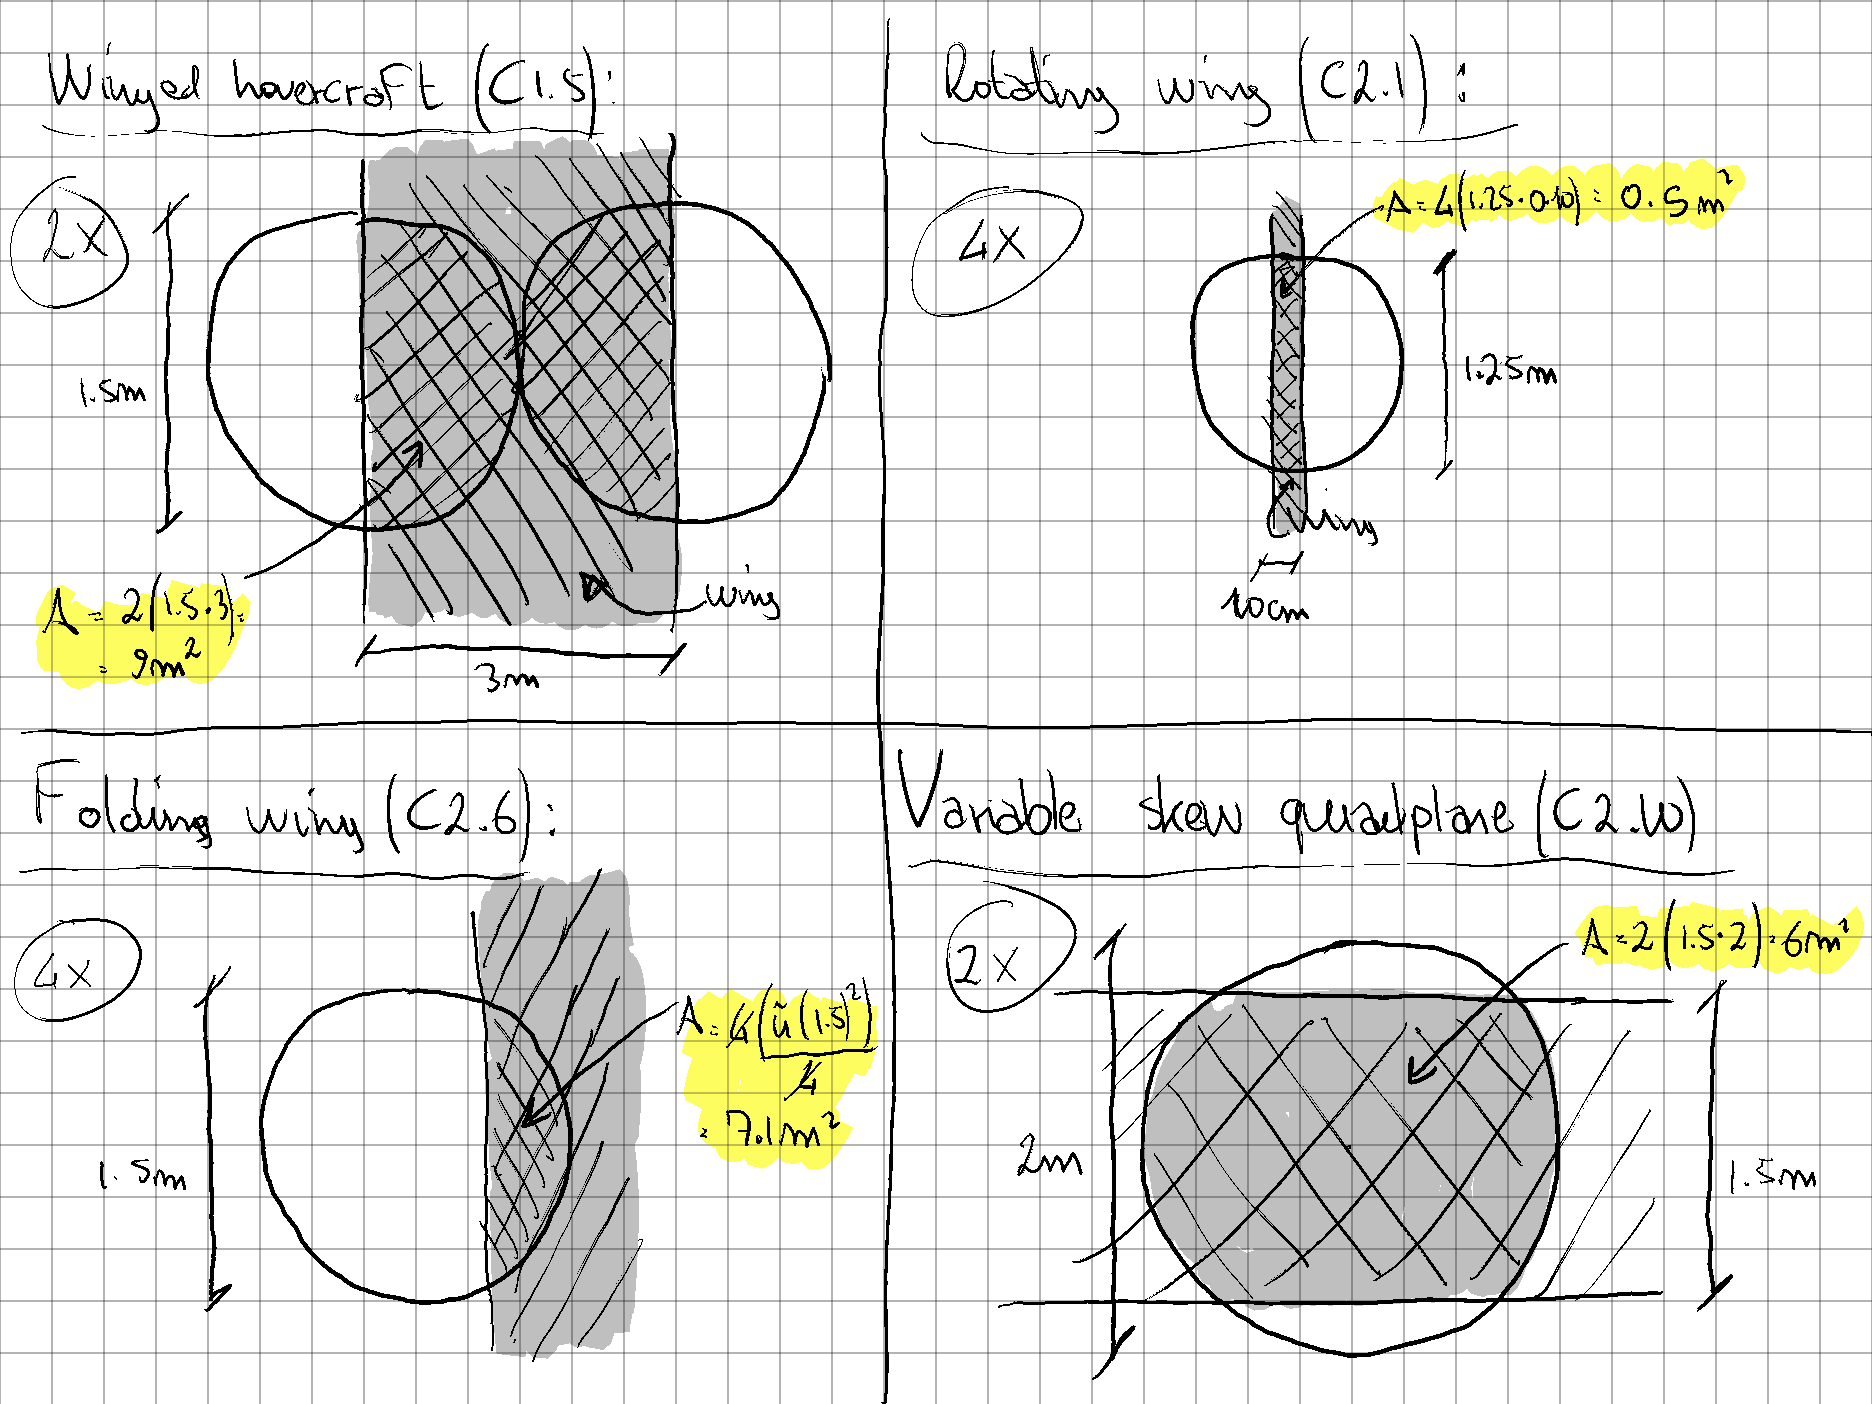
\includegraphics[width=0.75\linewidth]{figures/aeronoiseSKETCH.png}
    \caption{Sketches of engines obstruction per design}
    \label{fig:aeronoiseSKETCH}
\end{figure}


\section{Trade-Off Execution}
\label{sec:performtoff}
All the results from the earlier sections are assembled in the final trade-off table, \Cref{tab:performtoff}.
Here the final score for each design is computed, and the winning concept ultimately determined.
Criteria are assigned to columns, where relative widths are proportional to the criteria weights, for ease of visualisation and interpretation. 
Whereas concepts are assigned to rows.
Scores are indicated in parentheses in each cell, next to a brief score explanation. 
It is strongly encouraged to look at the various criteria sections for more details on scoring.
The final score is ultimately computed by means of a weighted average and presented in the right-most column as a decimal figure.
\begin{longtable}[c]{p{2.8cm}|p{1.1cm}|p{2.1cm}|p{1.5cm}|p{1.8cm}|p{1.1cm}|p{1.5cm}|c}
\caption{Final trade-off}
\label{tab:performtoff}\\
\diagbox[width=3.2cm]{\textbf{Concepts}}{\textbf{Criteria}}
                         & \textbf{CR-01} & \centering \textbf{CR-02} & \centering \textbf{CR-03} & \centering \textbf{CR-04} & \centering \textbf{CR-05} & \centering \textbf{CR-06} & \textbf{Final Score}\\ \hline
\endfirsthead
%
\endhead
%
\ref{C1.5} (Winged   Rotorcraft) & \cellcolor[HTML]{83C77D}Full-sized model (4)    & \cellcolor[HTML]{E0E383}Excellent control, low CEF\footnote{conversion effectiveness factor} (3)   & \cellcolor[HTML]{E0E383}6 moving parts, low complexity, low loads (3)   & \cellcolor[HTML]{83C77D}Energy consumption  67.0 kWh (4) & \cellcolor[HTML]{63BE7B}Full redundancy (5) & \cellcolor[HTML]{E0E383}Engine noise  122.7 dB, obstruction area  9$\text{m}^2$ (3) & \cellcolor[HTML]{b2d580} \textbf{3.5}\\ \hline
\ref{C2.1} (Rotating Wing) & \cellcolor[HTML]{E0E383}Scale model highly tested (3)  & \cellcolor[HTML]{63BE7B}Good control, excellent CEF (5)            & \cellcolor[HTML]{E0E383}2 moving parts, low complexity, high loads (3)     & \cellcolor[HTML]{E0E383}Energy consumption  73.2 kWh (3) &\cellcolor[HTML]{E0E383}Fatal hinge failure (3)&    \cellcolor[HTML]{83C77D}Engine noise  125.2 dB, obstruction area  0.5$\text{m}^2$ (4)   &  \cellcolor[HTML]{9ace7e} \textbf{3.8}         \\ \hline
\ref{C2.6} (Folding Wing) & \cellcolor[HTML]{83C77D}Full-sized model (4)  & \cellcolor[HTML]{E0E383}High control, low CEF (3)            & \cellcolor[HTML]{FCBF7B}6 moving parts, high complexity,  medium loads (2)     & \cellcolor[HTML]{83C77D}Energy consumption  66.9 kWh (4) &\cellcolor[HTML]{63BE7B}Full redundancy (5)&    \cellcolor[HTML]{E0E383}Engine noise  120.6 dB, obstruction area  7.1$\text{m}^2$ (3)   &\cellcolor[HTML]{c9dc82} \textbf{3.4}           \\ \hline
\ref{C2.10} (Variable Skew Quad Plane) & \cellcolor[HTML]{FCBF7B}Scale model (2)  & \cellcolor[HTML]{E0E383}High control, low CEF (3)            & \cellcolor[HTML]{83C77D}1 moving part, low complexity, medium loads (4)     & \cellcolor[HTML]{FCBF7B}Energy consumption  78.4 kWh (2) &\cellcolor[HTML]{83C77D}Fail-safe (4)&    \cellcolor[HTML]{FCBF7B}Engine noise  134.2 dB, obstruction area  6$\text{m}^2$ (2)     &\cellcolor[HTML]{eed17f} \textbf{2.8}         \\


% Final score              & \cellcolor[HTML]{E0E383}3.5 & \cellcolor[HTML]{83C77D}3.75 & \cellcolor[HTML]{E0E383}3.35 & \cellcolor[HTML]{FCBF7B}2.8
\end{longtable}


%%final toff table but with scores only (for presentation)
% \begin{longtable}[c]{p{2.8cm}|p{1.1cm}|p{2.1cm}|p{1.5cm}|p{1.8cm}|p{1.1cm}|p{1.5cm}|p{1.1cm}}
% \caption{Final trade-off table}
% \label{tab:performtoff}\\
% \diagbox[width=3.2cm]{Concepts}{Criteria}
%                          & CR-01 & \centering CR-02 & \centering CR-03 & \centering CR-04 & \centering CR-05 & \centering CR-06 & Final score\\ \hline
% \endfirsthead
% %
% \endhead
% %
% C1.5 (Winged   Rotorcraft) & \cellcolor[HTML]{83C77D}(4)    & \cellcolor[HTML]{E0E383}(3)   & \cellcolor[HTML]{E0E383}(3)   & \cellcolor[HTML]{83C77D}(4) & \cellcolor[HTML]{63BE7B}(5) & \cellcolor[HTML]{E0E383}(3) & \cellcolor[HTML]{b2d580} \textbf{3.5}\\ \hline
% C2.1 (Rotating Wing) & \cellcolor[HTML]{E0E383}(3)  & \cellcolor[HTML]{63BE7B}(5)            & \cellcolor[HTML]{E0E383}(3)     & \cellcolor[HTML]{E0E383}(3) &\cellcolor[HTML]{E0E383}(3)&    \cellcolor[HTML]{83C77D}(4)   &  \cellcolor[HTML]{9ace7e} \textbf{3.75}         \\ \hline
% C2.6 (Folding Wing) & \cellcolor[HTML]{83C77D}(4)  & \cellcolor[HTML]{E0E383}(3)            & \cellcolor[HTML]{FCBF7B}(2)     & \cellcolor[HTML]{83C77D}(4) &\cellcolor[HTML]{63BE7B}(5)&    \cellcolor[HTML]{E0E383}(3)   &\cellcolor[HTML]{c9dc82} \textbf{3.35}           \\ \hline
% C2.10 (Variable Skew Quad Plane) & \cellcolor[HTML]{FCBF7B}(2)  & \cellcolor[HTML]{E0E383}(3)            & \cellcolor[HTML]{83C77D}(4)     & \cellcolor[HTML]{FCBF7B}(2) &\cellcolor[HTML]{83C77D}(4)&    \cellcolor[HTML]{FCBF7B}(2)     &\cellcolor[HTML]{eed17f} \textbf{2.8}         \\ 


% % Final score              & \cellcolor[HTML]{E0E383}3.5 & \cellcolor[HTML]{83C77D}3.75 & \cellcolor[HTML]{E0E383}3.35 & \cellcolor[HTML]{FCBF7B}2.8
% \end{longtable}


\begin{longtable}[c]{lllll}
\label{tab:trade-off_Legend}\\
\multicolumn{5}{c}{\textbf{Legend}} \\
\endfirsthead
%
\endhead
%
\bottomrule
\multicolumn{1}{l|}{\cellcolor[HTML]{FD6864}Poor} &
  \multicolumn{1}{l|}{\cellcolor[HTML]{FCBF7B}Low} &
  \multicolumn{1}{l|}{\cellcolor[HTML]{E0E383}Medium} &
  \multicolumn{1}{l|}{\cellcolor[HTML]{A2D07F}High} &
  \cellcolor[HTML]{63BE7B}Excellent
\\\toprule
\end{longtable}

As it can be seen in \Cref{tab:performtoff}, the trade-off is won by concept \ref{C2.1}, the Rotating Wing, with an overall score of 3.8.
The Rotating Wing concept is therefore selected as the best, most suitable to perform the required mission.
To validate the trade-off, a sensitivity analysis will be performed in \Cref{ch:SensitivityAnalysis}.


% \section{Trade Off Summary table}
% \label{sec:TradeOffSummaryTable}
